% Created 2019-07-01 lun. 17:36
\documentclass[11pt]{article}
\usepackage[utf8]{inputenc}
\usepackage[T1]{fontenc}
\usepackage{fixltx2e}
\usepackage{graphicx}
\usepackage{longtable}
\usepackage{float}
\usepackage{wrapfig}
\usepackage{rotating}
\usepackage[normalem]{ulem}
\usepackage{amsmath}
\usepackage{textcomp}
\usepackage{marvosym}
\usepackage{wasysym}
\usepackage{amssymb}
\usepackage{hyperref}
\tolerance=1000
\date{\today}
\title{Replay Detection}
\hypersetup{
  pdfkeywords={},
  pdfsubject={},
  pdfcreator={Emacs 25.3.1 (Org mode 8.2.10)}}
\begin{document}

\maketitle
\tableofcontents




\section{{\bfseries\sffamily TODO} : Problématique}
\label{sec-1}
\subsection{Replay}
\label{sec-1-1}
\subsubsection{Pourquoi les replays}
\label{sec-1-1-1}
\subsubsection{Logo}
\label{sec-1-1-2}

\section{Objectif}
\label{sec-2}
Nous voulons comparer l'efficacité des méthodes de vision par ordinateur "classique"
aux méthodes par apprentissage profond (deep learning).
L'objectif dans cette parti est double. Le premier est de détecter le plus efficacement les
logos dans les vidéos afin d'avoir une \textbf{base line} à comparer avec l'approche par deep learning. 
Le second est de mettre en place un système capable d'extraire les
frames avec des logo, et ce sans intervention humaine (pas de labeling, pas d'ensemble d'entraînement
à construire), afin de pouvoir constituer automatiquement un ensemble de données permettant d'entraîner
des modèles de machine learning.


\section{Première partir : Détection sans deep learning}
\label{sec-3}
\section{Détection des replays : êtat de l'art}
\label{sec-4}
\subsection{A Robust Replay Detection}
\label{sec-4-1}
Cette approche détecte les replays en trouvant les logos dans la vidéo.
Les logos sont trouvés grâce à la luminance. Nous savons qu'un logo est présent pendant 0.8 secondes soit 18 frames pour une vidéo de 24 FPS. 
Tous les frames qui ont obtenu un score supérieur à un certain seuil sont considérés comme des "logo templates".

\subsubsection{Calcul du score de la luminance et filtrage des frames}
\label{sec-4-1-1}
L'idée est de parcourir toute la vidéo et de calculer pour chaque frame
la différence de luminance qu'il y a entre ce frame et les 17 frames précédents. 
Nous obtenons un score L$_{\text{i}}$ pour chaque frame i dans la vidéo.
Tous les frames dont le score est inférieur à un certain seuil sont écartés,
les autres vont servir à trouver le logo template.

\subsubsection{Recherche du logo template parmis les frames filtrés}
\label{sec-4-1-2}
Le logo template est le frame qui représente le mieux tous les logos dans la
vidéo. Pour déterminer le logo template parmis les frames filtrés, l'algorithme
K-means est utilisé pour séparer cet ensemble en deux (K = 2) en fonction de la
luminance moyenne des frames. Pour trouver le logo template, nous allons 
chercher dans le cluster avec le centre de cluster le plus élevé, le frame m
minimisant la distance avec tous les autres frames N du cluster. 

\subsubsection{Recherche des logo}
\label{sec-4-1-3}
Une fois que le logo template est déterminé, chaque logo trouvé en 1 va être 
comparé avec le logo template. La mesure de comparaison est la distance qu'il 
y a entre le frame et le template dans le cluster.
Tous les frames qui ont une distance inférieure à un certain threshold sont 
considérés comme des logos.

\subsubsection{Recherche des replays}
\label{sec-4-1-4}
Une fois que les logos sont détectés, nous pouvons trouver les replays en 
cherchant les paires de logos éloignés de moins de 80 seconde (durée 
maximum d'un replay).

\subsubsection{Conclusion sur cette méthode}
\label{sec-4-1-5}
Trop dépendant de la luminance, ne parvient pas à détecter les logo 
peu lumineux. 
Peu précis (trop de faux positif)
Dépend de trop de paramètres (seuil de luminance, \ldots{}) affectant 
les logos détectés.

\subsection{Fast Highlight Detection and Scoring for Broadcast Soccer Video Summarization using On-Demand Feature Extraction and Fuzzy Inference}
\label{sec-4-2}
\subsubsection{Idée}
\label{sec-4-2-1}
Entrainer un algorithme CART des histogrammes 3D sur des frames de logos choisi à la main.
Utilisé l'algorithme CART sur les histogrammes pour prédire logo/non-logo.

\subsubsection{Conclusion}
\label{sec-4-2-2}
Nous ne voulons pas maintenir un ensemble d’apprentissage. Cette méthode ne convient pas à nos besoins.

\subsection{Automatic summarization of soccer highlights using audio-visual descriptors}
\label{sec-4-3}
\subsubsection{Idée}
\label{sec-4-3-1}
S = Détecter tous les shots (plans) dans la vidéo 
L = Pour chaque shot S$_{\text{i}}$:
\begin{itemize}
\item L$_{\text{i}}$$_{\text{start}}$ = La "luminance" des frames au début du shot
\item L$_{\text{i}}$$_{\text{end}}$ = La "luminance" des frames à la fin du shot
\item L$_{\text{template}}$ = Trouver le "logo template" dans L
\item Pour chaque logo l dans L:
\begin{itemize}
\item Diff l avec L$_{\text{template}}$ = conversion grayscale puis somme de la soustraction pixel par pixel
\item Si Diff l avec L$_{\text{template}}$ < threshold => l est un logo
\end{itemize}
\end{itemize}

\subsubsection{Conclusion}
\label{sec-4-3-2}
Cette méthode est trop semblable à l’approche “Robust Replay Detection” qui ne répond pas à nos besoin, 
cette approche ne fonctionnera pas dans notre cas (la luminance n’est pas un critère assez discriminant
pour la reconnaissance de logo). Néanmoins, l’idée de découper la vidéo en “shot” (en plan) est
intéressante et nous nous en servons par la suite.

\subsection{MEAN SHIFT BASED VIDEO SEGMENT REPRESENTATION AND APPLICATIONS TO REPLAY DETECTION}
\label{sec-4-4}

\subsubsection{Idée}
\label{sec-4-4-1}
Segmenter la vidéo en frame, puis calculer une représentation compressée de chaque frame. 
Pour détecter les logo (ou n'importe quoi), il faut d'abord "apprendre" plusieurs formes
compressées de logo (sur des vidéos d'apprentissage que nous aurons labelisé à la main), 
puis il faut simplement calculer une distance entre la forme compressé du shot à définir
et les formes compressées apprises.

\subsubsection{Conclusion}
\label{sec-4-4-2}
Cette approche est intéressante, néanmoins l’article n’est pas assez précis, notamment 
sur la manière dont les images sont compressées. De plus, nous ne voulons par maintenir 
un ensemble d’apprentissage. Cette méthode ne convient donc pas à nos besoins.

\subsection{Real-time field sports scene classification using colour and frequency space decompositions}
\label{sec-4-5}
\subsubsection{Idée}
\label{sec-4-5-1}
Classifie les shots en fonction de la distance (proche, moyen, loin) et de ce qu'il y a 
dedans (visage, épaule, un seul joueur,  plusieurs joueurs, terrain, spectateur). 

\subsubsection{Conclusion}
\label{sec-4-5-2}
A l'air d'être une approche solide. Néanmoins, c'est de la classification supervisée,
il faut donc un ensemble d'apprentissage. Cette méthode ne convient donc pas à nos besoins.


\section{Les approches proposées}
\label{sec-5}
\subsection{{\bfseries\sffamily TODO} : mettre en avant le fait que l'algo va être mis en prod}
\label{sec-5-1}
Les méthodes "état de l'art" ne donnent pas d'assez bons résultats et ne peuvent 
pas être mises en production. Nous cherchons donc notre propre méthode.

Pour détecter les replays, nous faisons les hypothèses que :
\begin{itemize}
\item un replay a un logo de début (I)
\item un replay a un logo de fin (II)
\item les logos de début et de fin sont les mêmes (III)
\item les logos ont une forme facilement reconnaissable qui se distingue des  autres images dans la vidéo (IV)
\item un replay dure entre 2 et 90 secondes (V)
\end{itemize}

Nous proposons plusieurs approches permettant de détecter les logo de replay dans
les vidéo de sport. Dans cette partie, chacune de ces approches n'utilisent que des algorithmes
de computer vision classique (flouttage, filtre de Canny, ORB, \ldots{}) et des algorithmes de machine 
learning non-supervisés (K-NN).
Ces restrictions s'appliquent pour les raisons suivantes :
\begin{itemize}
\item le programme doit être le plus rapide possible (les réseaux de neurones sont en général trop lents,
trop exigeant en ressource); d'où le choix d'algorithme plus simple.
\item si la solution doit être mise en production, il est préférable de ne pas avoir d'ensemble d'apprentissage
à obtenir ou maintenir; d'où le choix d'algorithme non-supervisé uniquement.
\end{itemize}

\subsection{Détection des plans}
\label{sec-5-2}
Les approches que nous proposons itérent sur tous les frames de la vidéo, à la recherche des
logo pouvant se trouver au début et à la fin des replays. Si nous faisons l'hypothèse qu'un 
replay entraînera toujours un changement de plan, alors au lieu de rechercher les logo
parmi tous les frames de la vidéo, nous réduisons la recherche à tous les frames qui sont entre deux
plans.
\subsubsection{ONLINE, SIMULTANEOUS SHOT BOUNDARY DETECTION AND KEY FRAME EXTRACTION FOR SPORTS VIDEOS USING RANK TRACING}
\label{sec-5-2-1}
Cette méthode est proposée par W. Abd-Almageed en 2008.

Chaque frame est converti en HSV et les histogrammes H, S et V sont calculés. 
Un vecteur est formé pour chaque frame à partir de ces histogrammes.

Ensuite, une matrice M de dimension N * L, représentant une fenêtre de N frames va
être formée à partir de ces vecteurs, où L est la taille des histogrammes et N la taille de la fenêtre.

L'algorithme SVD (singular value decomposition) va être appliquée sur M. M = UWV, 
où W est la matrice de valeur singulière. 

Les diagonales de la matrice W comportent des poids S ordonnées de manière non croissante. 
Le premier poid S$_{\text{1}}$ est le poid maximal. Ces poids représentent l'information contenu dans le vecteur V.

Nous allons assigner un rang à la matrice M,  ce rang va être égal au nombre d'élement s dans S 
tel que s/S1 > threshold. Le rang va être calculé pour chaque fenêtre de frame dans la vidéo. 

Si le rang d'une fenêtre est plus que grand que le rang de la fenêtre avant elle, alors le 
contenu visuel de la fenêtre est différent de la fenêtre précédente. 
A l'inverse, si le rang est inférieure à la fenêtre précédente, 
alors le contenu visuel se stabilise. S'il est de 1, alors c'est stable.

Le début d'un frame est celui qui maximise le rang parmis les fenêtres environnantes.

\begin{enumerate}
\item Résultats obtenus et conclusion
\label{sec-5-2-1-1}
Cette méthode pour trouver les plans dans une vidéo est très efficace, et constitue la
base de la suite de notre recherche. 

En effet, avant de segmenter la vidéo en plan, nous comparions  N frames , où N peut être 
aussi grand que 400000 (pour des vidéo de 120 minutes à 60 fps), il est impensable d’utiliser 
un algorithme en O(N²), par exemple en comparant toutes les frames entre elles, avec un N aussi grand.

Après avoir segmenter la vidéo en plan, nous obtenons un N’ au alentours de 2000 pour une vidéo
de 120 minutes à 60 fps. Nous pouvons donc nous permettre d’utiliser des algorithmes plus 
complexes que sans la segmentation en plan.
De plus, la segmentation en plan réduit le champs de recherche des frames logo, 
et donc le nombre de faux positifs potentiels.
\end{enumerate}


\section{Première approche : ORB}
\label{sec-6}
Dans cette approche, nous cherchons à reconnaître les logo dans la vidéo.
Pour ce faire, nous optons pour une approche de clustering. L'idée 
est de clusteriser la vidéo en deux groupe : un groupe pour les frames 
logo, et un autre groupe pour les frames non-logo.

\subsection{Extraction des caractéristiques}
\label{sec-6-1}
OpenCV permet d'extraire des features à partir des images (détection des bords 
des objets dans l'image).
A partir de ça, nous pouvons représenter l'image comme un vecteur de feature.
Les méthodes d'extraction sont ORB et AKAZE.

\subsection{KMeans}
\label{sec-6-2}
OpenCV implémente aussi l'algorithme KMeans. Celui-ci permet de regrouper les
objets similaires en fonction de leur feature. Dans notre cas, il va nous 
permettre de créer 2 groupes d'images : logo / non logo.
L'avantage de KMeans est qu'il est est très rapide et assez efficace dans la
plupart des cas. C'est l'un des algorithmes de clusterisation les plus utilisés.


\subsection{Expérimentation et résultat:}
\label{sec-6-3}
Ensemble de test : une vidéo de ligue 1, une vidéo de liga, une vidéo de 
premier league et une vidéo NFL.
Dans toutes les expérimentations, la vidéo est découpée en shot (plan). 
Soit S l'ensemble des shots.

\subsection{1 frame par shot}
\label{sec-6-4}
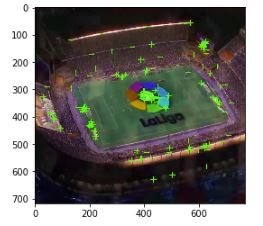
\includegraphics[width=.9\linewidth]{orb_simple_res.JPG}
\begin{itemize}
\item Récupérer le frame à la fin de chaque shot
\begin{itemize}
\item nous obtenons |S| frame
\end{itemize}
\item Pour chaque frame, calculer ses features (orb ou akaze)
\begin{itemize}
\item Nous obtenons |S| vecteurs
\end{itemize}
\item Utiliser KMeans avec K=2 pour séparer les vecteurs en deux groupes 
\begin{itemize}
\item le groupe le plus petit est le groupe des logo
\end{itemize}
\end{itemize}

Résultats : 
\subsubsection{{\bfseries\sffamily TODO} meilleurs res}
\label{sec-6-4-1}
Mauvais sur toutes les vidéos

\subsection{W frames par shot:}
\label{sec-6-5}
\begin{itemize}
\item Récupérer W frames pour chaque shot 
\begin{itemize}
\item nous obtenons |S*W| frame, où W est le nombre de frame
\end{itemize}
\item Pour chaque frame, calculer ses features (orb ou akaze) 
\begin{itemize}
\item nous obtenons |S*W| vecteurs
\end{itemize}
\item Utiliser KMeans avec K=2 pour séparer les vecteurs en deux groupes 
\begin{itemize}
\item le groupe le plus petit est le groupe des logo
\end{itemize}
\end{itemize}

Résultats : 
Mauvais sur toutes les vidéos

\subsection{1 fenêtre de frame par shot:}
\label{sec-6-6}
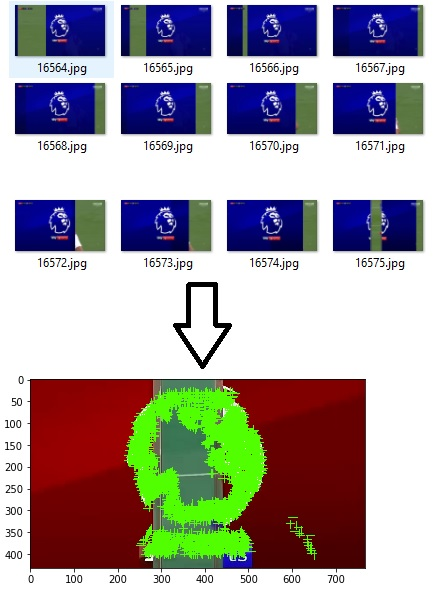
\includegraphics[width=.9\linewidth]{akaze_window_res.JPG}
\begin{itemize}
\item Récupérer W frames pour chaque shot, les régrouper en une fenêtre
\begin{itemize}
\item nous obtenons |S| fenêtre de dimension W, où W est le nombre de frame
\end{itemize}
\item Pour chaque fenêtre, calculer ses features (orb ou akaze) 
\begin{itemize}
\item Nous obtenons un vecteur de dimension |S*W|
\end{itemize}
\item Utiliser KMeans avec K=2 pour séparer les vecteurs en deux groupes 
\begin{itemize}
\item le groupe le plus petit est le groupe des logo
\end{itemize}
\end{itemize}

Résultats:
De bons résultats sur la vidéo de PL.
Mauvais résultats sur les autres vidéos.


\subsection{1 fenêtre de frame par shot et différence des frames dans la fenêtre:}
\label{sec-6-7}
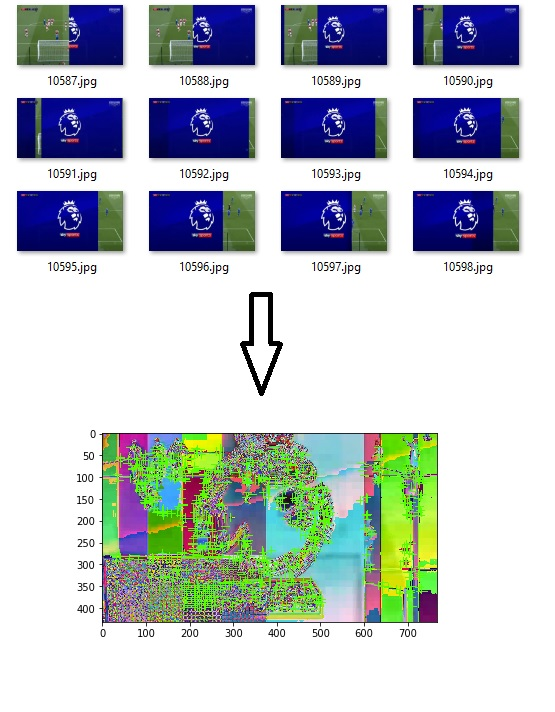
\includegraphics[width=.9\linewidth]{orb_window_diff_res.JPG}
\begin{itemize}
\item Récupérer W frames pour chaque shot, les régrouper en une fenêtre
\begin{itemize}
\item nous obtenons |S| fenêtre de dimension W, où W est le nombre de frame
\end{itemize}
\item Pour chaque fenêtre, calculer la matrice M égale à la différence de toute 
les autres frames dans la fenêtre
\item Pour chaque matrice de différence, calculer ses features
\begin{itemize}
\item nous obtenons |S| vecteur s
\end{itemize}
\item Utiliser KMeans avec K=2 pour séparer les vecteurs en deux groupes 
\begin{itemize}
\item le groupe le plus petit est le groupe des logo
\end{itemize}
\end{itemize}

Résultats :
De bons résultats sur la vidéo de PL.
Mauvais résultats sur les autres vidéos.


\section{Seconde approche : matching de contours}
\label{sec-7}
La méthode choisie différe avec les autres sur un point : au lieu de chercher
à différencier les frames logo des frames non-logo, nous allons chercher 
les frames qui ont des formes en commun dans la vidéo.
En effet, d'après l'hypothèse III, il est fort probable que si un frame à 
l'instant t a beaucoup de formes en commun avec un frame à l'instant t', avec 
2 < t' < 90 (hypothèse V), alors il y a un logo à l'instant t et un logo à 
l'instant t', et un replay entre t et '.
\subsection{Algorithme}
\label{sec-7-1}
\begin{itemize}
\item Pré traitement sur les shots
\begin{enumerate}
\item Redimensionner
\item Cropper
\item Supprimer le background (s’étendre la dessus)
\item Détecter le contour (Canny Edge Detection)
\item Génération des mosaiques TODO : explain this
\end{enumerate}
\item Pour chaque mosaique de plan S$_{\text{A}}$ :
\begin{itemize}
\item Pour chaque mosaique de plan S$_{\text{B}}$ après S$_{\text{A}}$ :
\begin{enumerate}
\item Contour$_{\text{commun}}$ = C$_{\text{A}}$ \& C$_{\text{B}}$
\item Contours$_{\text{diff}}$ = Détection du contour de Contour$_{\text{commun}}$ (cv2.findContours)
\item Résultat = Ne garder que les contours qui sont assez longs (ceux qui ont au moins K points)
\item Si Résultat > Seuil : alors S$_{\text{A}}$ et S$_{\text{B}}$ sont des logos potentiels
\end{enumerate}
\end{itemize}
\item Pour chaque logo potentiel LP :
\begin{enumerate}
\item Le comparer avec les autres logo L’ (même procédure qu’en 2)
\item Si au moins 2 logo L’  match, alors LP est un logo
\end{enumerate}
\item Trouver les replays grâce aux logos
\end{itemize}

Pré traitement :
Les frames sont resizé puis cropé vers le centre (pour ne pas avoir l'affichage
en haut de l'écran etc\ldots{}), puis un blur est appliqué (bilateralFilter, permet 
de filtrer certains faux positifs), et enfin on applique Canny Edge Detection.

Le point 3 de l’algorithme sert à filtrer les éventuels faux positifs. 
Notre algorithme est sensible au plan fixe et aux images avec beaucoup de bruits
(ces images ont beaucoup de contours détectés par l’algorithme de détection de contours). 
Beaucoup de ces faux-positifs peuvent être filtrer lors du pré-traitement sur les plans,
 notamment en rajoutant du blur ou en supprimant le background, néanmoins, nous ne sommes 
pas parvenus à filtrer 100\% des faux-positifs.

\subsection{Mosaique de plan}
\label{sec-7-2}
\subsubsection{{\bfseries\sffamily TODO} resize img}
\label{sec-7-2-1}
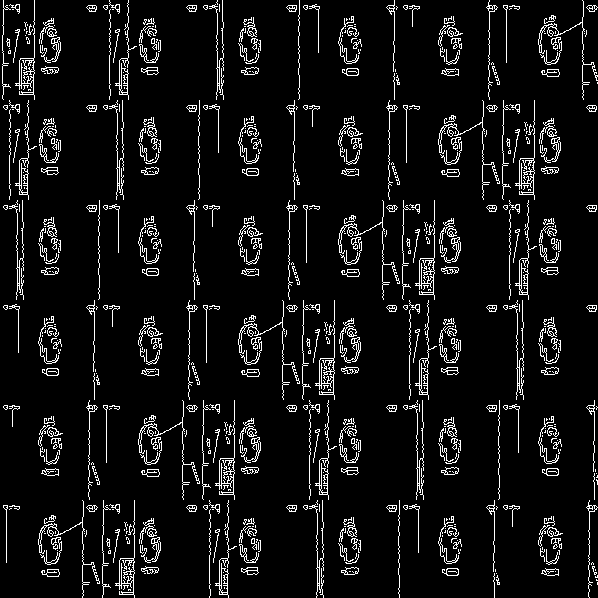
\includegraphics[width=.9\linewidth]{mosaique1.png}
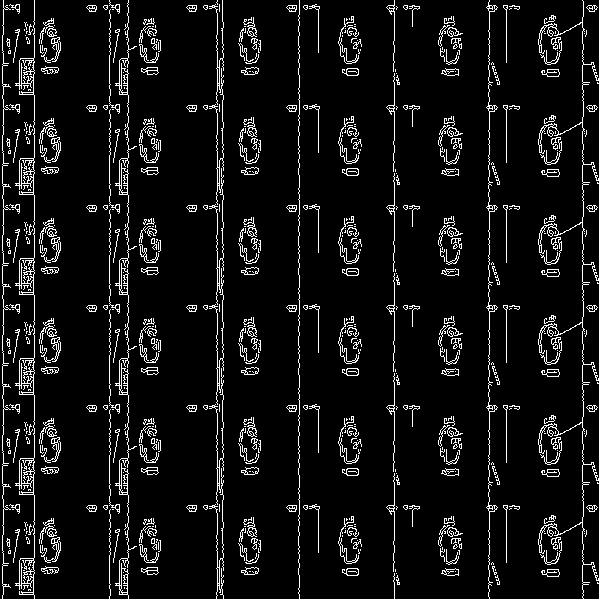
\includegraphics[width=.9\linewidth]{mosaique2.png}
Pour chaque shot deux images au format .png (pas au format jpg, car celui-ci prend trop d'espace disque) sont générées.

Chaque image est de dimension I * I * width * height où I est le nombre de frame dans le shot.

Ces images sont en faites des matrices d'image qui vont permettre de comparer rapidement deux shot.
La première matrice a un décalage d'un frame par ligne, la seconde n'a pas de décalage.

Pour comparer deux shot, il suffit d’appliquer un ET binaire entre les matrices des mosaiques, 
puis de calculer la longueur du conteur dans cette matrice.


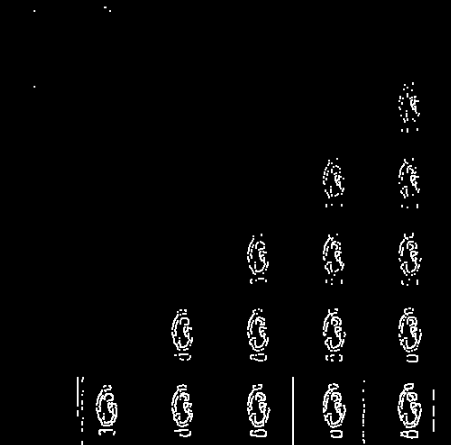
\includegraphics[width=.9\linewidth]{mosaique3.png}

\subsection{Résultats et limitation}
\label{sec-7-3}
Les résultats sans le filtrage des faux positifs (l’étape 3 de l’algorithme) sont un 
bon moyen d’évaluer l’efficacité de notre méthode. 
\subsubsection{{\bfseries\sffamily TODO} : mettre les résultats ici}
\label{sec-7-3-1}
Concernant le temps d’exécution, celui-ci est relié presque entièrement à la taille de
la vidéo donnée en entrée, ainsi qu’à la taille des mosaiques.

Les limitations de notre méthode sont les suivantes :
\begin{itemize}
\item Dans certaines vidéos, il n’y a pas de logo pour les replays (simple fondu)
\item Dans certaines vidéos, les logo de début et fin de replay ne sont pas les mêmes.
\item Dans certains vidéos, il y a des logo au début des replays, mais pas de logo à
la fin des replays (un simple fondu remplace le logo).
\end{itemize}



\section{Deuxième partie : Détection avec deep learning}
\label{sec-8}

\subsection{Etat de l'art}
\label{sec-8-1}
Nous nous intéressons à l'état de l'art concernant la détection d'action
dans les vidéos. En effet, la transition d'un logo s'effectue sur plusieurs 
frames consécutives; il y a donc une composante temporelle à notre recherche,
et nous pouvons considérer la transition d'un logo comme une action.
\subsubsection{Two-Stream Convolutional Networks for Action Recognition in Videos}
\label{sec-8-1-1}
Cet article est écrit par Karen Simonyan et Andrew Zisserman. Dans celui-ci,
ils proposent de séparer la tâche de reconnaissance d'action dans les vidéos en 
deux parties : une composante spatiale et une composante temporelle.
La composante spatiale contient l'information concernant sur les objets dans
la vidéo; tandis que la composante temporelle l'information sur les 
déplacements de ces objets et de la caméra. 
A partir de ces observations, les auteurs proposent d'entraîner un classifieur
spatial (Spatial stream ConvNet) et un classifieur temporel (). Ces classifieurs
sont des réseaux de neurones convolutifs profonds. 

\begin{enumerate}
\item Classifieur spatial
\label{sec-8-1-1-1}
Ce réseau a une architecture de classifieur d'image classique. Il va permettre
de donner un indice fort pour la prédiction, car certaines actions sont très 
liées à certains objets.

\item Classifieur temporel
\label{sec-8-1-1-2}
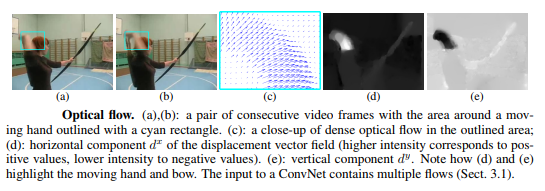
\includegraphics[width=.9\linewidth]{optical_flow.png}
Source : Two-Stream Convolutional Networks for Action Recognition in Videos, Figure 2
L'innovation de l'article vient de l'introduction du classifieur temporel.
L'idée est de détecter le mouvement des objets dans la vidéo, car un mouvement
est la représentation d'un objet dans le temps.
Les auteurs appellent leur approche "optical flow stacking".
Dans celle-ci ils utilisent la méthode "optical flow" pour détecter
le mouvement des objets entre des frames consécutives. 
Ces mouvements vont être stockés dans des vecteurs et utilisés par le classifieur.
Ils définissent aussi un hyperparamètre L qui définit la distance maximum entre deux frames
pour laquel il faut calculer l'optical flow. Par exemple, si L=5, alors pour le 
frame \#50, il faudra calculer l'optical flow entre le frame \#50 et le frame \#51; entre
\#50 et \#52; etc\ldots{} jusqu'à \#50 à \#55.

\item Méthode d'évalutation et résultats obtenus
\label{sec-8-1-1-3}
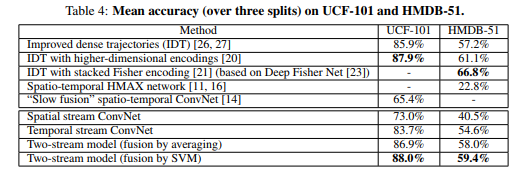
\includegraphics[width=.9\linewidth]{two_stream_res.png}
Source : Table 4: Mean accuracy (over three splits) on UCF-101 and HMDB-51.

Le classifieur spatial est pré-entrainé avec ImageNet, tandis que le temporel
est entraîné de zéro (car il n'y a pas de réseau déjà entraîné pour cette tâche).
Les dataset utilisés pour l'entraînement et l'évaluation sont UCF-101 et HMDB-51,
contenant à eux deux près de 20000 vidéos annotées.

\textbf{Note} Pour calculer la classe d'un frame à l'instant t, les auteurs proposent
deux méthodes :
\begin{itemize}
\item fusion par la moyenne (by averaging) : y$_{\text{t}}$ = y$_{\text{t}}$$_{\text{spatial}}$ + y$_{\text{t}}$$_{\text{temporal}}$ / 2
\item fusion par SVM (by SVM) : un SVM multiclasse linéaire est entrainé pour
\end{itemize}
prédire la classe à partir du softmax des scores L2-normalisés.

Les résultats en \textbf{link table} montrent l'efficacité de leur méthode par rapport
aux autres approches état de l'art.

Nous pouvons voir que leur approche two-stream avec fusion SVM est la plus 
efficace sur le dataset UCF-101, et qu'elle a aussi de bons résultats sur
HMDB-51.

Ce qui est le plus intéressant dans cet article, c'est l'amélioration
qu'apporte l'ajout de la composante temporelle.
En effet, le classifieur d'image simple (spatial) n'a que 73.0\% (UCF-101) et 
40.5\% (HMBD-51), tandis que le classifieur qui prend en compte l'image et 
la temporalité (two-stream model) atteint \textbf{88.0\%} et 59.4\%; ce qui 
est une nette amélioration. Cet article nous a renforcé dans l'hypothèse
qu'il est nécessaire d'étudier une vidéo non pas comme une suite d'image 
indépendante, mais comme une suite de séquence avec un lien au sein de 
chaque séquence.
Il semblerai que la temporalité a une très grande importance pour 
l'analyse de vidéos.
\end{enumerate}

\subsubsection{Temporal Segment Networks: Towards Good Practices for Deep Action Recognition}
\label{sec-8-1-2}
ConvNet ne peut pas être appliquée à la reconnaîssance d'action dans les vidéos pour deux raisons :
\begin{itemize}
\item Les dépendances temporelles éloignées jouent un rôle important dans la compréhension des actions dans les vidéos.
\end{itemize}
Or, les réseaux ConvNet classiques se focalisent sur les dépendances proches (les mouvements brefs).
\begin{itemize}
\item Entraîner un réseau de type ConvNet requiert un gros volume de données pour obtenir des performances optimales.
\end{itemize}
Or, obtenir des ensembles de données annotées et de qualité est une tâche compliquée; le sur apprentissage est un
problème important à considérer.


\subsection{Scrapping}
\label{sec-8-2}
L'approche par matching de contours convient tout à fait à la tâche de scrapping.
En effet, elle est :
\begin{itemize}
\item rapide : moins de \textbf{X} minutes sur une machine \textbf{machine de référence EC2 (ou autre)} pour une vidéo de 90 minutes à 60 fps
\item précise : seulement \textbf{X} \% de faux positifs sur \textbf{Y} logos scrappés
\end{itemize}

\subsubsection{Architecture du scrapper}
\label{sec-8-2-1}
\begin{itemize}
\item requête HTTP avec une ID youtube => logo uploadé sur GCP
\item image docker (avec le serveur à l'écoute des requêtes) déployée sur le cloud
\end{itemize}
Cette architecture est scalaire; ceci nous a permi de scrapper plusieurs vidéos en parallèle et d'obtenir un dataset conséquent.

\subsection{Datasets}
\label{sec-8-3}
\begin{itemize}
\item Dataset non logo
\item Dataset logo
\item Dataset logo séparé en fonction du logo (ligue 1, premier league, \ldots{})
\end{itemize}


\subsection{Détection des frames logo}
\label{sec-8-4}
\subsubsection{Propre modèle}
\label{sec-8-4-1}
\subsubsection{VGG net}
\label{sec-8-4-2}
\subsubsection{Transfert Learning}
\label{sec-8-4-3}
\subsubsection{Comparaison résultat}
\label{sec-8-4-4}

\subsection{Détection des séquences de frames logo}
\label{sec-8-5}

\section{Appendice}
\label{sec-9}
Clustering :
Histogramme : 
Frame : 
Shot : plan
FPS : frame per second / image par seconde
Cropper

\section{Source}
\label{sec-10}
Two-Stream Convolutional Networks for Action Recognition in Videos, Karen Simonyan Andrew Zisserman, 2014
% Emacs 25.3.1 (Org mode 8.2.10)
\end{document}
